%!TEX root = main.tex

\chapter{Formulações lineares inteiras para o problema da árvore $t$-spanner de peso mínimo}
\label{cap:mwstp}
Neste capítulo abordamos o problema da árvore $t$-spanner de
peso mínimo (MWTSP). Mais especificamente, apresentamos duas
formulações lineares inteiras que propusemos para o MWTSP. Estas são
as primeiras formulações específicas para este problema (no sentido de
não serem formulações para o problema de $t$-spanners adaptadas para
árvores).  Inicialmente mencionamos outras definições equivalentes à
definição de $t$-spanner apresentada no
Capítulo~\ref{cap:introducao}, uma das quais será utilizada nas
formulações apresentadas neste e no próximo capítulo.  Depois
apresentamos uma heurística que pode ser utilizada no caso de peso
unitário. Posteriormente, apresentamos uma formulação linear baseada
no uso de arborescências. Na Seção~\ref{sec:form_mwstp_lab_dist},
apresentamos outra formulação linear para o MWTSP também baseada no
uso de arborescências, mas com variáveis específicas que capturam a
noção de distância.
%{\color{red}Por fim, na Seção~\ref{sec:publicacoes}, apresentamos as
%  publicações resultantes (principalmente) deste capitulo.}

\section{Outras definições equivalentes de $t$-spanner}

% Cai e Corneil \cite{CaiC1995} mostraram que várias definições de $t$-spanner são equivalentes. 
% Para a formulação que apresentaremos, o seguinte resultado é importante.

% Seja $Q$ um subgrafo gerador conexo de $G$.  A seguinte definição é equivalente à definição~(\ref{eq:def_spanner}):
% \begin{equation}
% \dist_{Q}(u,v) \le t \cdot \dist_{G}(u,v), \quad \forall\;uv \in E.
% \label{eq:def2_spanner}
% \end{equation}



% \smallskip

% A prova de que (\ref{eq:def_spanner}) implica (\ref{eq:def2_spanner}) 
% é direta. Vamos provar que (\ref{eq:def2_spanner}) implica (\ref{eq:def_spanner}). 

% \begin{observacao}
% \label{obs:relate_spanner_definitions}
% Seja $Q$ um subgrafo gerador conexo de $G$. Então
% \begin{equation*}
% \begin{split}
% \dist_{Q}(u,v) \le t \cdot  \dist_{G}(u,v), \forall\;uv \in E \implies \\
% \dist_{Q}(u,v) \le t \cdot \dist_{G}(u,v), \forall\;u,v \in V.
% \end{split}
% \end{equation*}
% \begin{proof}
% Sejam $u,v \in V$. Se $uv \in E$, por hipótese, segue a conclusão. 
% Vamos assumir que $uv \notin E$. Seja 
% $P = (u = u_0, u_1, \ldots, u_{\ell-1}, u_{\ell} = v)$ um caminho de peso mínimo entre 
% $u$ e $v$ em $G$. Por hipótese, para cada \\
% \mbox{$u_{i-1}u_i \in E(P), \dist_{Q}(u_{i-1},u_i) \le t \cdot \dist_{G}(u_{i-1},u_i)$}.
%  Então
% \begin{align*}
% \dist_{Q}(u,v) &\le \sum_{i = 1}^{\ell} dist_{Q}(u_{i-1},u_i)\\ 
% &\le \sum_{i = 1}^{\ell} t \cdot  \dist_{G}(u_{i-1},u_i)\\
% &= t \cdot \sum_{i = 1}^{\ell} \dist_{G}(u_{i-1},u_i)\\
% &= t \cdot \dist_{G}(u,v),
% \end{align*}
% onde a última igualdade segue do fato de que a distância entre $u$
% e $v$ em $G$ é igual à soma das distâncias entre os vértices
% consecutivos que compõem um caminho de peso mínimo entre $u$ e $v$ em $G$. 
% % o custo de um caminho de custo mínimo é igual ao somatório do custo das 
% % arestas que compoem o 
% % caminho.
% \end{proof}
% \end{observacao}
Cai e Corneil~\cite{CaiC1995}  mostraram algumas definições de $t$-spanner equivalentes à definição apresentada
no Capítulo~\ref{cap:introducao}. Para a formulação que
apresentamos na Seção \ref{sec:formulacao}, os seguintes resultados são úteis.

\begin{lema}
  \label{lem:definicoes}
  Seja $G = (V,E)$ um grafo conexo com peso
\hbox{$w: E \to \espacoRpos$,} e $t \ge 1$ um número real. 
Seja $H$ um subgrafo gerador de $G$. 
As seguintes afirmações são equivalentes:

\begin{itemize}
  \item[{\rm (a)}] $H$ é um $t$-spanner de $G$, isto é, $H$ satisfaz
    (\ref{eq:def_spanner});

  \item[{\rm (b)}] $\dist_{H}(u,v) \le t \cdot \dist_{G}(u,v) \;\forall\,uv \in E$;

  \item[{\rm (c)}] $\dist_{H}(u,v) \le t \cdot w_{uv} \;\forall\,uv \in E$.
    %% \begin{equation}
    %%   \dist_{Q}(u,v) \le t \cdot \dist_{G}(u,v), \quad \forall\;uv \in E.
    %%   \label{eq:def2_spanner}
    %% \end{equation}
\end{itemize}
\end{lema}

\begin{proof}
  A prova de que \rm (a) implica \rm (b) 
  é direta. Vamos provar que \rm (b) implica~\rm (a). Isto é, 

%%   \label{obs:relate_spanner_definitions}
%% Seja $Q$ um subgrafo gerador conexo de $G$. Então
\begin{equation*}
\begin{split}
\dist_{H}(u,v) \le t \cdot  \dist_{G}(u,v)\; \forall\,uv \in E\implies \\
\dist_{H}(u,v) \le t \cdot \dist_{G}(u,v) \; \forall\,u,v \in V.
\end{split}
\end{equation*}
%% \begin{proof}
Sejam $u,v \in V$. É suficiente provarmos a desigualdade para o caso em que $uv \notin E$. Seja 
$P = (u = u_0, u_1, \ldots, u_{\ell-1}, u_{\ell} = v)$ um caminho de peso mínimo entre 
$u$ e $v$ em $G$. Por hipótese, para cada 
$u_{i-1}u_i \in E(P)$, temos que $\dist_{H}(u_{i-1},u_i) \le t \cdot \dist_{G}(u_{i-1},u_i)$.
 Então
\begin{align*}
\dist_{H}(u,v) &\le \sum_{i = 1}^{\ell} dist_{H}(u_{i-1},u_i)\\ 
&\le \sum_{i = 1}^{\ell} t \cdot  \dist_{G}(u_{i-1},u_i)\\
&= t \cdot \sum_{i = 1}^{\ell} \dist_{G}(u_{i-1},u_i)\\
&= t \cdot \dist_{G}(u,v),
\end{align*}
onde a última igualdade segue do fato de que a distância entre $u$
e $v$ em $G$ é igual à soma das distâncias entre os vértices
consecutivos que compõem um caminho de peso mínimo entre $u$ e $v$ em $G$. 
% o custo de um caminho de custo mínimo é igual ao somatório do custo das 
% arestas que compoem o 
% caminho.
%% \end{proof}

A prova de que (\rm a) implica (\rm c) é imediata. Vamos provar que (\rm c) implica (\rm a). Considere $u,v \in V$, e tome um caminho de peso mínimo de $u$ a $v$, digamos $P$, em $G$. Seja $xy$ uma aresta de $P$: \begin{itemize}
  \item Se $xy \in E(H)$, então $\dist_{H}(x,y) \le w_{xy} \le t \cdot w_{xy}$;
  \item Se $xy \not\in E(H)$, então $\dist_{H}(x,y) \le t \cdot w_{xy}$ (por hipótese).
\end{itemize}
Portanto, $\dist_{H}(u,v) \le \sum_{xy \in E(P)} dist_{H}(x,y) \le t \cdot \sum_{xy \in E(P)} w_{xy} = t \cdot \dist_{G}(u,v)$.
\end{proof}


%%%%%%%%%%%%%%%%%%%%%%%%%%%%%%%%%%%%%%%%%


\section{Heurística para o caso unitário}
\label{sec:mwsp_preprocessamento}
Dado um grafo $G = (V,E)$, onde $|V| = n$, uma função peso 
$w: E \to \conjInteirosPos$, e um inteiro $2 \le D \le n - 2$,  
o problema da \emph{árvore geradora mínima com diâmetro limitado} (do 
inglês \emph{Bounded Diameter Minimum Spanning Tree Problem} - BDMSTP) 
tem por objetivo encontrar uma árvore geradora de peso mínimo cujo número
de arestas no caminho entre quaisquer dois vértices seja no máximo $D$. 
%% é 
%% definido como: dado um grafo $G = (V,E)$, onde $|V| = n$, uma função peso 
%% $w: E \to \mathbb{Z}^+$, e um inteiro $2 \le D \le n - 2$, o objetivo é 
%% encontrar uma árvore geradora de peso mínimo cujo número de arestas no 
%% caminho entre quaisquer dois vértices seja no máximo $D$.
É sabido que a 
versão de decisão deste problema é NP-completo \cite{GareyJ1990}. 

Se o peso das arestas é unitário, o BDMSTP pode ser resolvido em tempo
polinomial (no tamanho de $G$) \cite{GareyJ1990}.
Neste caso, temos uma heurística que, caso seja bem-sucedida na
  busca de uma solução viável, tal solução é ótima para o MWTSP
  (considerando $t = D$).
Para resolver o BDMSTP no caso unitário,
podemos executar o algoritmo de busca em largura~\cite{CormenLRS2009}
a partir de
cada um dos vértices de $G$ até que, para um determinado vértice,
a altura da árvore de busca (de $G$) não seja maior do que
$h = \floor{D / 2}$. Caso $h$ seja ímpar, consideramos cada dois vértices
(adjacentes) ao invés de um como centro, realizamos a contração da aresta
representada pelos dois vértices e executamos o algoritmo de busca em largura
a partir deste vértice criado. Havendo solução, a árvore final deverá conter
a aresta contraída.

%% Vamos apresentar a seguir um algoritmo (descrito em
%% \cite{Nadiradze2013}) para resolver o problema para o caso unitário.

%% Considere uma solução ótima $T^{*}$ para o BDMSTP.
%% Seja $p$ um caminho de $T^*$ com o maior número de arestas. 
%% Se $D$ é par, seja o vértice $c$ o centro de $p$. Se $D$ é ímpar, seja 
%% $cc'$ a aresta central de $p$. Seja $r = \floor{D / 2}$. Observe que, 
%% se $D$ é par, para cada vértice $v \in V$, o número de arestas entre $v$ e 
%% $c$ é no máximo $r$. Caso $D$ seja ímpar, o número de arestas entre $v$ e 
%% $c$ ou entre $v$ e $c'$ é no máximo $r$.

%% O algoritmo seguinte resolve o BDMSTP para o caso unitário. Seja $c$ um
%% vértice de $V$. Caso 
%% $D$ seja ímpar, seja $cc'$ uma aresta de $G$. O vértice $c$ será considerado o 
%% centro da nossa solução e, caso $D$ seja ímpar, $c'$ também será um centro.
%% Marcamos o(s) centro(s) como vértice(s) já adicionado(s). 
%% Fazemos uma busca em largura em somente um nível a partir do(s) centro(s) e,
%% para cada vizinho
%% não marcado $x$, nós adicionamos a aresta selecionada ($cx$ ou, se for o caso,
%% $c'x$) à solução final e marcamos o vértice $x$ como adicionado.

%% Nós repetimos o processo para os novos vértices até que o número de arestas 
%% do caminho entre o centro $c$ e os vértices adicionados não seja maior do que
%% $r$ (caso $D$ seja ímpar, tomamos o mesmo cuidado para o centro $c'$). 
%% Se todos os vértices 
%% foram marcados ao final, nós temos uma solução ótima. Caso contrário, iniciamos 
%% uma nova rodada escolhendo outro(s) vértice(s) como centro e repetimos o 
%% algoritmo. Observe que cada rodada em questão corresponde ao algoritmo de busca 
%% em largura. Sendo assim, a complexidade total do algoritmo é 
%% $O((|V| + |E|) \cdot |V|)$ \cite{CormenLRS2009}.

\section{Formulação SR: encontrando distâncias entre os vértices}
\label{sec:form_mwstp}

\begin{figure}
  \centering
\begin{tikzpicture}%
  [%>=stealth,
   %shorten >=1pt,
    node distance=2cm,
   auto%,
  ]
  
          \tikzstyle{every state}=[
            draw = black,
            thick,
            fill = white,
            minimum size = 4mm
        ]
  
\node[state] (l1)                  {};
\node[state] (l2) [below left of=l1] {};
\node[state] (l3) [below right of=l1] {};
\node[state] (l4) [below left of=l2] {};
\node[state] (l5) [below right of=l2] {};
\node[state] (l6) [below right of=l3] {};
\node[state] (l7) [below left of=l5] {};
\node[state] (l8) [below right of=l5] {};
\node[left] at (l4.west){$G$:};

\path[]
%   FROM       BEND/LOOP           POSITION OF LABEL   LABEL   TO
   (l1)     edge     node                    {} (l2)
           edge     node                    {} (l3)
    (l4)    edge     node                    {} (l2)
    (l2)    edge     node                    {} (l5)
    (l3)    edge     node                    {} (l5)
    (l3)    edge     node                    {} (l6)
    (l5)    edge     node                    {} (l7)
    (l5)    edge     node                    {} (l8)
    (l4)    edge     node                    {} (l7)
    (l6)    edge     node                    {} (l8)
   ;
\end{tikzpicture}
\qquad
\begin{tikzpicture}%
  [>=stealth,
   %shorten >=1pt,
   node distance=2cm,
   auto%,
  ]

\tikzset{myptr/.style={decoration={markings,mark=at position 0.5 with %
      {\arrow[scale=2,>=stealth]{>}}},postaction={decorate}}}
  
  
          \tikzstyle{every state}=[
            draw = black,
            thick,
            fill = white,
            minimum size = 4mm
        ]
  
\node[state] (l1)                  {};
\node[state] (l2) [below left of=l1] {};
\node[state] (l3) [below right of=l1] {};
\node[state] (l4) [below left of=l2] {};
%\node[state] (l5) [label=right:$b_1$,below right of=l2] {};
\node[state] (l5) [below right of=l2] {};
\node[state] (l6) [below right of=l3] {};
\node[state] (l7) [below left of=l5] {};
\node[state] (l8) [below right of=l5] {};
\node[left] at (l4.west){$D$:};

\path[]
%   FROM       BEND/LOOP           POSITION OF LABEL   LABEL   TO
   (l1)     edge[bend left, myptr]     node                    {} (l2)
           edge[bend left, myptr]     node                    {} (l3)
    (l2)   edge[bend left, myptr]      node                    {} (l1)
    (l3)   edge[bend left, myptr]     node                    {} (l1)
    (l4)    edge[bend left, myptr]     node                    {} (l2)
    (l2)    edge[bend left, myptr]     node                    {} (l4)
    (l2)    edge[bend left, myptr]     node                    {} (l5)
    (l5)    edge[bend left, myptr]     node                    {} (l2)
    (l3)    edge[bend left, myptr]     node                    {} (l5)
    (l5)    edge[bend left, myptr]     node                    {} (l3)
    (l3)    edge[bend left, myptr]     node                    {} (l6)
    (l6)    edge[bend left, myptr]     node                    {} (l3)
    (l5)    edge[bend left, myptr]     node                    {} (l7)
    (l7)    edge[bend left, myptr]     node                    {} (l5)
    (l5)    edge[bend left, myptr]     node                    {} (l8)
    (l8)    edge[bend left, myptr]     node                    {} (l5)
    (l4)    edge[bend left, myptr]     node                    {} (l7)
    (l7)    edge[bend left, myptr]     node                    {} (l4)
    (l6)    edge[bend left, myptr]     node                    {} (l8)
    (l8)    edge[bend left, myptr]     node                    {} (l6)
   ;
\end{tikzpicture}
\caption{{Grafo $G$ e o correspondente digrafo $D$}}
\label{fig:digrafo_ini}
\end{figure}


%% \begin{figure}[t]
%%   \centering
%%   %\input{figures/xfig/arb_diferentes}
%%   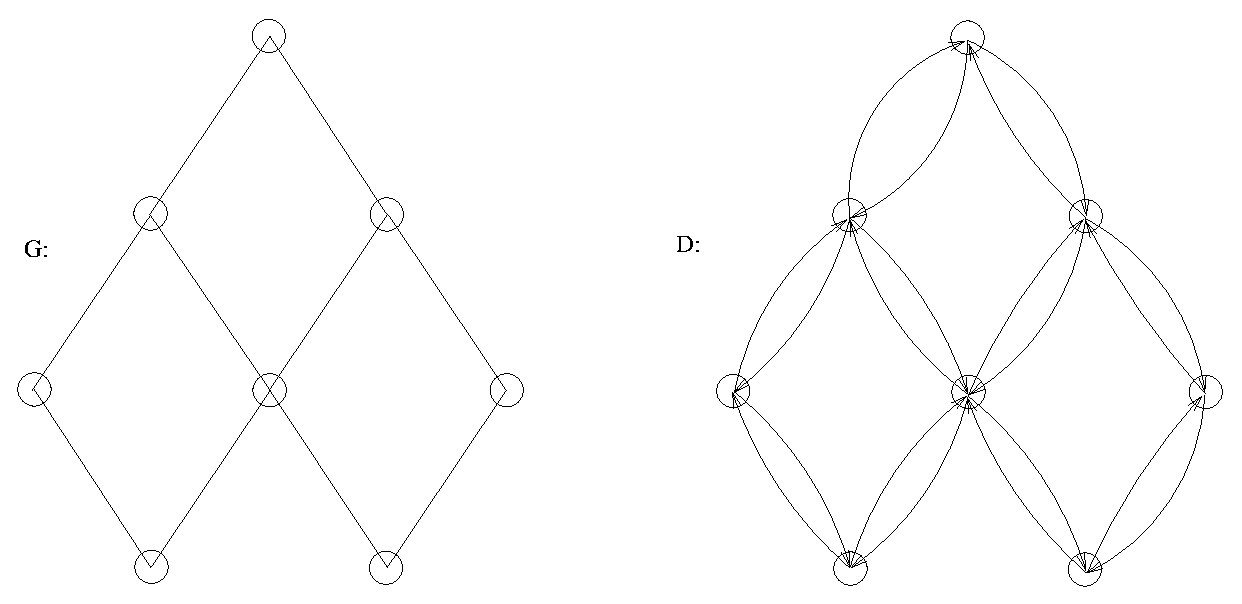
\includegraphics[scale=0.55]{figuras/digrafo_ini}
%%   \caption{Digrafo relacionado ao grafo original}
%%   \label{fig:digrafo_ini}
%% \end{figure}

Nesta seção, vamos apresentar uma formulação linear inteira para o
problema de árvores $t$-spanner baseada no uso de arborescências.
Para trabalhar com arborescências, a partir do grafo dado $G$
construímos inicialmente um digrafo $D$.  Fazendo uso de
arborescências enraizadas em cada um dos vértices do digrafo~$D$,
podemos impor condições para que essas arborescências, quando
``sobrepostas'', definam uma árvore geradora em $G$. Isto nos permite
distinguir (facilmente), para cada par $u$, $v$ de vértices, quais são
as arestas que pertencem ao caminho entre $u$ e $v$ em tal
árvore. Isto ficará mais claro a seguir.

% Vamos inicialmente montar um sistema linear tal que, para cada solução deste
% sistema, tal solução representa uma árvore geradora de $G$. Além disso,
% neste sistema linear, para cada par $u,v \in V$, o objetivo é que 
% seja fácil distinguir quais são as arestas que pertencem
% ao caminho entre $u$ e $v$ nesta árvore.}


Dado um grafo conexo $G = (V,E)$, seja $D = (V,A)$ o digrafo obtido a
partir de~$G$, onde $A = \{(u,v),(v,u)\; |\; uv \in E\}$
(veja Figura~\ref{fig:digrafo_ini}).
%Usamos a notação $A(D)$ para denotar o conjunto de arcos do digrafo $D$.
Fixe um vértice
$v \in V$ (raiz),  considere $z^{v} = (z_{ij}^{v})_{ij \in A}$, e as seguintes
restrições:
%% \begin{align*}
%%   z^{v} = (z_{ij}^{v})_{ij \in A}.
%%   \end{align*}

\begin{lpformulation}[]
\lpeq[res_mwstp:single_in-arc]{\sum_{i \in \delta^{-}(j)}z^{v}_{ij} = 1}{j \in V \setminus \{v\}}
\lpeq[res_mwstp:root]{\sum_{i \in \delta^{-}(v)}z^{v}_{iv} = 0}{}
\lpeq[res_mwstp:int_z]{z^{v}_{ij} \in \{0,1\}}{ij \in A}
\lplabel{lp:tree_restriction}
\end{lpformulation}

A restrição~(\ref{res_mwstp:single_in-arc}) impõe que para cada
vértice~$j$ distinto de~$v$ seja selecionado exatamente um arco 
que chega em $j$. A restrição~(\ref{res_mwstp:root}) impõe que não
seja selecionado nenhum arco que chega em $v$.

Seja $\tilde{z}^{v}$ um ponto que satisfaz o sistema acima. Seja
$T^{v} \subseteq D$ tal que $A(T^{v}) = \{ij \in A\; |\; \tilde{z}^{v}_{ij} = 1\}$,
ou seja, $T^{v}$ é o digrafo de $D$ formado pelos arcos selecionados,
conforme as restrições acima. É imediato que vale o seguinte resultado.


\begin{figure}
  \centering
\begin{tikzpicture}%
  [>=stealth,
   %shorten >=1pt,
   node distance=2cm,
   auto%,
  ]

\tikzset{myptr/.style={decoration={markings,mark=at position 0.5 with %
      {\arrow[scale=2,>=stealth]{>}}},postaction={decorate}}}
  
  
          \tikzstyle{every state}=[
            draw = black,
            thick,
            fill = white,
            minimum size = 4mm
        ]
  
\node[state] (l1) [label=right:$v$]                  {};
\node[state] (l2) [below left of=l1] {};
\node[state] (l3) [below right of=l1] {};
\node[state] (l4) [below left of=l2] {};
%\node[state] (l5) [label=right:$b_1$,below right of=l2] {};
\node[state] (l5) [below right of=l2] {};
\node[state] (l6) [label=right:$w$,below right of=l3] {};
\node[state] (l7) [below left of=l5] {};
\node[state] (l8) [below right of=l5] {};
\node[left] at (l4.west){$T^{v}$:};

\path[]
%   FROM       BEND/LOOP           POSITION OF LABEL   LABEL   TO
   (l1)     edge[bend left, myptr]     node                    {} (l2)
    (l2)    edge[bend left, myptr]     node                    {} (l4)
    (l5)    edge[bend left, myptr]     node                    {} (l3)
    (l3)    edge[bend left, myptr]     node                    {} (l6)
    (l8)    edge[bend left, myptr]     node                    {} (l5)
    (l4)    edge[bend left, myptr]     node                    {} (l7)
    (l6)    edge[bend left, myptr]     node                    {} (l8)
   ;
\end{tikzpicture}
\qquad
\begin{tikzpicture}%
  [>=stealth,
   %shorten >=1pt,
   node distance=2cm,
   auto%,
  ]

\tikzset{myptr/.style={decoration={markings,mark=at position 0.5 with %
      {\arrow[scale=2,>=stealth]{>}}},postaction={decorate}}}
  
  
          \tikzstyle{every state}=[
            draw = black,
            thick,
            fill = white,
            minimum size = 4mm
        ]
  
\node[state] (l1) [label=right:$v$]                  {};
\node[state] (l2) [below left of=l1] {};
\node[state] (l3) [below right of=l1] {};
\node[state] (l4) [below left of=l2] {};
%\node[state] (l5) [label=right:$b_1$,below right of=l2] {};
\node[state] (l5) [below right of=l2] {};
\node[state] (l6) [label=right:$w$,below right of=l3] {};
\node[state] (l7) [below left of=l5] {};
\node[state] (l8) [below right of=l5] {};
\node[left] at (l4.west){$T^{w}$:};

\path[]
%   FROM       BEND/LOOP           POSITION OF LABEL   LABEL   TO
   (l1)     edge[bend left, myptr]     node                    {} (l2)
    (l3)   edge[bend left, myptr]     node                    {} (l1)
    (l2)    edge[bend left, myptr]     node                    {} (l4)
    (l3)    edge[bend left, myptr]     node                    {} (l5)
    (l6)    edge[bend left, myptr]     node                    {} (l3)
    (l5)    edge[bend left, myptr]     node                    {} (l8)
    (l4)    edge[bend left, myptr]     node                    {} (l7)
   ;
\end{tikzpicture}
\caption{Subgrafos $T^v$ e $T^w$}
\label{fig:arb_diferentes}
\end{figure}

%% \begin{figure}[t]
%%   \centering
%%   %\input{figures/xfig/arb_diferentes}
%%   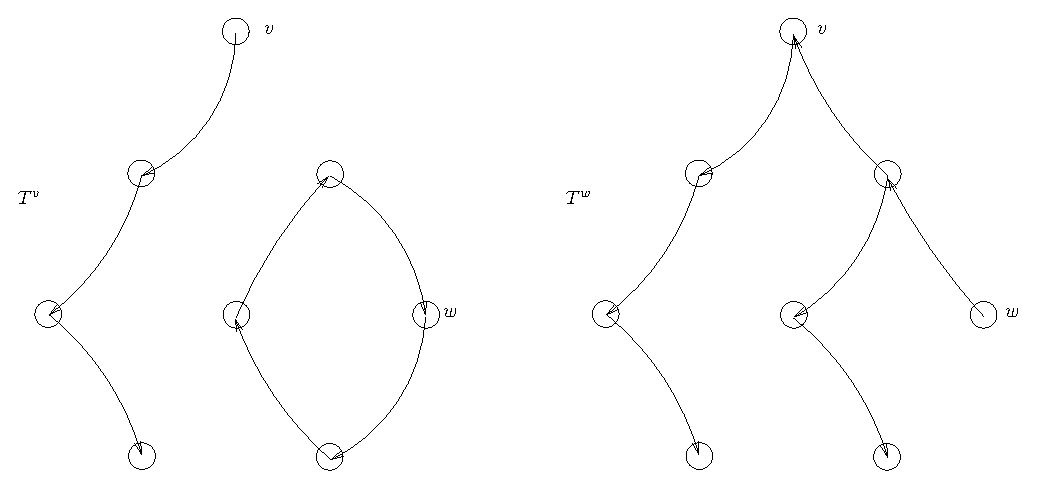
\includegraphics[scale=0.55]{figuras/arb_diferentes}
%%   \caption{Subgrafo formado pelos arcos selecionados}
%%   \label{fig:arb_diferentes}
%% \end{figure}


\begin{fato}
  \label{afirm:num_arcos}
  O subgrafo $T^{v}$ tem exatamente $|V| - 1$ arcos.
\end{fato}
Figura \ref{fig:arb_diferentes} ilustra possibilidades
para $T^{v}$ e $T^{w}$, onde $v$ e $u$ são vértices de $V$. 

Estamos interessados nos subconjuntos $F \subseteq E$ tais
  que $G[F]$ é uma árvore $t$-spanner de $G$. Em outras palavras,
o poliedro das árvores $t$-spanners de um grafo $G=(V,E)$, para um número real $t \ge 1$, é
definido como

\begin{equation*}
\begin{split}
P_{tree}(G,t) :=  \text{conv}\{\incid^{F} \in \espacoE, F \subseteq E\; |\; \text{$G[F]$ é uma árvore $t$-spanner\}}. 
\end{split}
\end{equation*}
%Seja $\incid^{F} \in P_{tree}(G,t)$. 

Vamos agora apresentar uma formulação linear inteira que descreve o
poliedro $P_{tree}(G,t)$.  Para isso, associamos a cada aresta $e$ em
$E$ uma variável $x_e$ com o seguinte significado: $x_e = 1$ se e só
se $e$ faz parte da solução.

As restrições sobre $x = (x_e)_{e \in E}$ são impostas fazendo uso das 
restrições vistas anteriormente --- para os subgrafos $T^v$ ---, definidas
para cada vértice $v$ do grafo $G$. 

%Vamos relacionar os subgrafos $T^{v}$ utilizando duas novas restrições
%juntamente com as restrições acima:
%Considere as seguintes inequações que relacionam os subgrafos $T^{v}$:

\begin{lpformulation}[]
\lpeq[res_mwstp:single_in-arc2]{\sum_{i \in \delta^{-}(j)}z^{v}_{ij} =
  1}{v \in V,\, \forall j \in V \setminus \{v\}}
\lpeq[res_mwstp:root2]{\sum_{i \in \delta^{-}(v)}z^{v}_{iv} = 0}{v\in V}
\lpeq[res_mwstp:single_arc]{x_e = z^{v}_{ij} + z^{v}_{ji}}{v \in V,\, \forall e = ij \in E}
\lpeq[res_mwstp:int_z2]{z^{v}_{ij} \in \{0,1\}}{v\in V,\, ij \in A}
\lpeq[res_mwstp:int_x]{x_e \in \{0,1\}}{e \in E}
\lplabel{lp:relate_arbs}
\end{lpformulation}
    Este sistema linear foi inspirado no trabalho de Conforti,
      Cornu{\'{e}}jols e
      Zambelli~\cite{ConfortiCZ2013}
      que trata do problema de 
      %% que tinham por objetivo obter uma forma
      %% diferente de
      representar o fecho convexo dos vetores de inciência das árvores
geradoras de um grafo.

\medskip

Seja $(\tilde{x},\tilde{z})$ uma solução do sistema acima. 
Como definimos anteriormente, para cada  $v \in V$, seja  $T^v$ 
o digrafo tal que $A(T^{v}) = \{ij \in A \; |\; \tilde{z}^{v}_{ij} = 1\}$, e seja
$\widetilde{T}^{v} \subseteq G$ o grafo subjacente
a $T^{v}$ tal que \mbox{$E(\widetilde{T}^{v}) = \{ij \in E\; |\; ij \in A(T^{v}) \text{ ou }ji
  \in A(T^{v})\}$}.

Não é difícil verificar as seguintes afirmações:


% Então, em decorrência da afirmação (\ref{afirm:arc_exist}), podemos
% concluir que

\begin{align}
  \label{afirm:same_arbs}
  \widetilde{T}^{v} = \widetilde{T}^{w}, \: \forall v, w \in V; 
\end{align}

\begin{align}
  \label{afirm:arborescence}
  T^{v} \text{ é uma arborescência de }D, \text{ com raiz }v, \: \forall v \in V.
\end{align}


A afirmação~(\ref{afirm:same_arbs}) é garantida pelas
restrições~(\ref{res_mwstp:single_arc}).

Suponha que a afirmação~(\ref{afirm:arborescence}) não seja correta. Suponha que exista
um vértice $u \in V$ para o qual exista um circuito em $\widetilde{T}^{u}$. Note que
$u$ não está contido em nenhum circuito de $\widetilde{T}^{u}$, caso contrário
violaria a restrição~(\ref{res_mwstp:root2}). 
Seja $v \in V$ tal que $v$ pertence  a um circuito $C_{v}$ de
$\widetilde{T}^{u}$. Em $T^v$, não existem dois arcos entrando em $v$, caso
contrário a restrição~(\ref{res_mwstp:root2}) seria violada.
Se considerarmos os dois caminhos direcionados a partir de $v$ em
$\{ij \in A(T^v)\; | \; \{i,j\} \in E(C_{v}) \}$, existirá um vértice
$w \in V(C_{v})$ tal que ambos os caminhos se encontram em $w$.
Então a restrição~(\ref{res_mwstp:single_in-arc2}) é violada para o vértice
$w$, uma contradição.

A partir das observações feitas acima, podemos concluir o seguinte
  fato relacionado ao sistema linear apresentado anteriormente. 

\begin{figure}[t]
  \centering
\begin{tikzpicture}%
  [>=stealth,
   %shorten >=1pt,
   node distance=2cm,
   auto%,
  ]

\tikzset{myptr/.style={decoration={markings,mark=at position 0.5 with %
      {\arrow[scale=2,>=stealth]{>}}},postaction={decorate}}}
  
  
          \tikzstyle{every state}=[
            draw = black,
            thick,
            fill = white,
            minimum size = 4mm
        ]
  
\node[state] (l1) [label=left:$v$]                  {};
\node[state] (l2) [below left of=l1] {};
\node[state] (l3) [below right of=l1] {};
\node[state] (l4) [below left of=l2] {};
%\node[state] (l5) [label=right:$b_1$,below right of=l2] {};
\node[state] (l5) [below right of=l2] {};
\node[state] (l6) [label=right:$w$,below right of=l3] {};
\node[state] (l7) [below left of=l5] {};
\node[state] (l8) [below right of=l5] {};
\node[left] at (l4.west){$T^{v}$:};

\path[]
%   FROM       BEND/LOOP           POSITION OF LABEL   LABEL   TO
   (l1)     edge[dashed, bend left, myptr]     node                    {} (l2)
    (l1)   edge[bend left, myptr]     node                    {} (l3)
    (l2)    edge[dashed, bend left, myptr]     node                    {} (l4)
    (l3)    edge[dashed, bend left, myptr]     node                    {} (l5)
    (l3)    edge[bend left, myptr]     node                    {} (l6)
    (l5)    edge[dashed, bend left, myptr]     node                    {} (l8)
    (l4)    edge[dashed, bend left, myptr]     node                    {} (l7)
   ;
\end{tikzpicture}  
\qquad
\begin{tikzpicture}%
  [>=stealth,
   %shorten >=1pt,
   node distance=2cm,
   auto%,
  ]

\tikzset{myptr/.style={decoration={markings,mark=at position 0.5 with %
      {\arrow[scale=2,>=stealth]{>}}},postaction={decorate}}}
  
  
          \tikzstyle{every state}=[
            draw = black,
            thick,
            fill = white,
            minimum size = 4mm
        ]
  
\node[state] (l1) [label=right:$v$]                  {};
\node[state] (l2) [below left of=l1] {};
\node[state] (l3) [below right of=l1] {};
\node[state] (l4) [below left of=l2] {};
%\node[state] (l5) [label=right:$b_1$,below right of=l2] {};
\node[state] (l5) [below right of=l2] {};
\node[state] (l6) [label=right:$w$,below right of=l3] {};
\node[state] (l7) [below left of=l5] {};
\node[state] (l8) [below right of=l5] {};
\node[left] at (l4.west){$T^{w}$:};

\path[]
%   FROM       BEND/LOOP           POSITION OF LABEL   LABEL   TO
   (l1)     edge[dashed, bend left, myptr]     node                    {} (l2)
    (l3)   edge[bend left, myptr]     node                    {} (l1)
    (l2)    edge[dashed, bend left, myptr]     node                    {} (l4)
    (l3)    edge[dashed, bend left, myptr]     node                    {} (l5)
    (l6)    edge[bend left, myptr]     node                    {} (l3)
    (l5)    edge[dashed, bend left, myptr]     node                    {} (l8)
    (l4)    edge[dashed, bend left, myptr]     node                    {} (l7)
   ;
\end{tikzpicture}
  \caption{Arborescências $T^u$ e $T^v$ se sobrepondo}
  \label{fig:arb_iguais}
\end{figure}


%% \begin{figure}[t]
%%   \centering
%%   %\input{figures/xfig/arb_diferentes}
%%   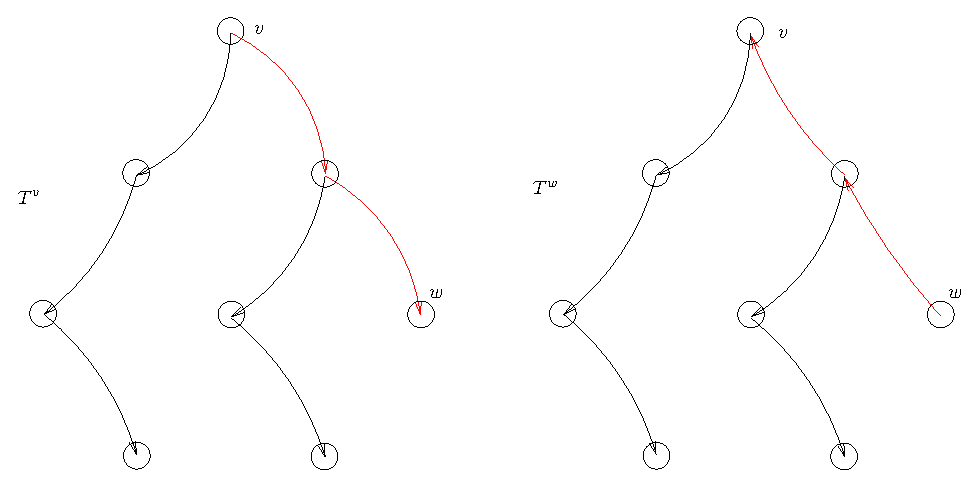
\includegraphics[scale=0.55]{figuras/arb_iguais}
%%   \caption{Arborescências se sobrepondo}
%%   \label{fig:arb_iguais}
%% \end{figure}



% Então, para $e = ij \in E$,
% temos que
% \begin{align}
%   \label{afirm:arc_exist}
%   x_e = 1 \Leftrightarrow ij \in T^{v} \oplus ji \in T^{v}, \forall v \in V.
% \end{align}


% \begin{align}
%   \label{afirm:same_arbs}
%   \widetilde{T}^{v} = \widetilde{T}^{w}, \: \forall v, w \in V;
% \end{align}

% \noindent de onde segue que 

% \begin{align}
%   \label{afirm:no_circuits}
%   T^{v} \text{ não tem circuitos}, \: \forall v \in V.
% \end{align}

% Seja $v \in V$. Suponha, por absurdo, que a afirmação acima não seja
% verdadeira e que exista um circuito $C$ em $T^v$.  Neste caso,
% quando tomarmos como raiz um vértice em $C$, a
% restrição~(\ref{res_mwstp:root2}) será violada para algum vértice em
% $C$.  A afirmação~(\ref{afirm:no_circuits}) juntamente com o
% fato~\ref{afirm:num_arcos} implica que

% \begin{align}
%   \label{afirm:arborescence}
%   T^{v} \text{ é uma arborescência de }D, \text{ com raiz }v, \: \forall v \in V.
% \end{align}

\medskip

\begin{fato}
  \label{afirm:arv_geradora}
  Seja $T \subseteq G$ tal que $E(T) = \{e \in E \; |\; x_e = 1\}$. Então $T$
  é uma árvore geradora de~$G$, e $T=\widetilde{T}^{v}$ para todo
  $v\in V$.
\end{fato}
Figura \ref{fig:arb_iguais} mostra duas arborescências que se ''sobrepõem''.


\medskip

Como dito anteriormente,
a formulação acima foi feita com o propósito de facilitar distinguir,
para cada par de vértices $u,v$ em $G$, quais são as arestas que
pertencem ao caminho de $u$ a $v$ na árvore $T$ (acima definida).
Precisamos identificar tais caminhos para impor a condição sobre o
fator de dilatação. Para isso, vamos definir novas variáveis de decisão.

É importante observar que, como todas as arborescências têm como
grafo subjacente a árvore $T$, quando tomamos dois vértices
distintos em $T$, digamos $u$ e~$v$, as arborescências $T^u$ e $T^v$
diferem apenas na orientação dos arcos no caminho de $u$ a $v$.  
Mais precisamente, na arborescência $T^u$ há um caminho orientado
de $u$ a $v$; e
na arborescência $T^v$ há um caminho orientado de $v$ a $u$. Os 
arcos que não pertencem ao caminho de $u$ a $v$ têm a mesma
orientação tanto em $T^u$ quanto em $T^v$. Este fato (ilustrado na 
Figura \ref{fig:arb_iguais}) é central para as 
as restrições que apresentaremos a seguir.
%% Figura \ref{fig:arb_iguais} ilustra este fato.

Para cada aresta $f\in E$, considere $y^{f} = (y^{f}_{e})_{e \in E}$. 
A variável $y\in \espacoY$ tem o seguinte significado: para cada
aresta $e\in E$, e cada aresta $f = uv \in E$, queremos que
$y^{f}_{e} = 1$ se e somente se a aresta $e$ pertence ao caminho entre
$u$ e $v$ em~$T$.

Note que na definição da variável $y$, só consideramos os pares de
vértices que definem aresta, em vez de considerarmos todos os pares de
vértices. Estamos usando aqui a equivalência garantida no
Lema~\ref{lem:definicoes}.%, conforme comentamos no capítulo anterior.

Para todo $uv, ij \in E$, considere as seguintes definições, feitas
para poder distinguir a pertinência de $ij$ nas arborescências $T^u$ e $T^v$:
\begin{align*}
  d^{u v}_{ij} := z^{u}_{ij} - z^{v}_{ij}\\
  s^{u v}_{ij} := z^{u}_{ij} + z^{v}_{ij}\\
  \end{align*}
\vspace{-1.5cm}
\small
\begin{center}
  \noindent
  \captionof{table}{Diferenças e somas relativas à variável $z$}
  \label{tab:sum_diff}
  \medskip
  
\begin{tabular}{|r|r|r|r|}\hline
{$d^{uv}_{ij}$ $s^{uv}_{ij}$} & {$z^{u}_{ij}$ $z^{v}_{ij}$} & {$z^{u}_{ji}$ $z^{v}_{ji}$} & {$d^{uv}_{ji}$ $s^{uv}_{ji}$}
\\ \hline\hline 
$1\quad 1$ & $1\quad 0$ & $0\quad 1$ & $-1\quad 1$ \\
$-1\quad 1$ & $0\quad 1$ & $1\quad 0$ & $1\quad 1$ \\
$0\quad 2$ & $1\quad 1$ & $0\quad 0$ & $0\quad 0$ \\
$0\quad 0$ & $0\quad 0$ & $1\quad 1$ & $0\quad 2$ \\
$0\quad 0$ & $0\quad 0$ & $0\quad 0$ & $0\quad 0$ \\
\hline\hline
\end{tabular}
\end{center}

\bigskip

%% Para $uv \in E$, seja $T_{u,v}$ o caminho entre $u$ e $v$ na árvore
%% $T$. %%definição está na introdução

As quatro primeiras linhas da Tabela \ref{tab:sum_diff} representam
os casos nos quais $ij \in E(T)$, enquanto que na quinta linha,
$ij \notin E(T)$. Para $u,v \in V(T)$, seja $T_{u,v}$ o caminho entre $u$ e $v$
em $T$. Nas duas primeiras linhas, $ij \in E(T_{u,v})$,
enquanto que na terceira e na quarta, $ij \notin
E(T_{u,v})$
  Considerando o caminho $T_{u,v}$, 
  os valores apresentados nas quatro primeiras linhas se devem a dois fatos: 
  cada arco em $T^u$ (referente a este caminho) está no sentido contrário do arco análogo em $T^v$; 
  os demais arcos de $T^u$ estão no mesmo sentido que os análogos em $T^v$.


  \hfill
  
Considere as seguintes inequações:
%
\begin{lpformulation}[]
  \lpeq[res_mwstp:define_y_ij]{d^{uv}_{ij} \le y^{uv}_{e} \le s^{uv}_{ij}} {uv \in E, \forall e = \{i,j\} \in E}
  \lpeq[res_mwstp:define_y_ji]{d^{uv}_{ji} \le y^{uv}_{e} \le s^{uv}_{ji}} {uv \in E, \forall e = \{i,j\} \in E}
\end{lpformulation}

Pela Tabela \ref{tab:sum_diff} e pelas inequações
(\ref{res_mwstp:define_y_ij}) e (\ref{res_mwstp:define_y_ji}), podemos
concluir que para todo $uv \in E$ e todo $e \in E$, temos que
%
\begin{align}
  \label{afirm:valor_y}
  y^{uv}_e = 1 \Leftrightarrow e \in E(T_{u,v}).
\end{align}

%\newpage

Juntando todas a restrições mencionadas, obtemos a seguinte
formulação, denominada \emph{sem rótulos} (SR), para o MWTSP.

%\begin{absolutelynopagebreak}
  \begin{lpformulation}[{\rm (PA)}]
    \lpobj*{min}{\sum_{e\in E} w_ex_e}
    \lpeq[res_mwstp:num_aresta]{\sum_{e \in E}x_e = |V| - 1}{}
    \lpeq[]{\sum_{i \in \delta^{-}(j)}z^{v}_{ij} = 1}{v \in V,\,\forall j \in V \setminus \{v\}}
    \lpeq[]{\sum_{i \in \delta^{-}(v)}z^{v}_{iv} = 0}{v \in V}
    \lpeq[]{x_e = z^{v}_{ij} + z^{v}_{ji}}{v \in V,\, \forall e = \{i,j\} \in E}
    \lpeq[]{z^{u}_{ij} - z^{v}_{ij} \le y^{uv}_{e} \le z^{u}_{ij} + z^{v}_{ij}} {uv \in E,\, \forall e = \{i,j\} \in E}
    \lpeq[]{z^{u}_{ji} - z^{v}_{ji} \le y^{uv}_{e} \le z^{u}_{ji} + z^{v}_{ji}} {uv \in E,\, \forall e = \{i,j\} \in E}
    \lpeq[]{\sum_{e \in E} w^{}_e\,y^{uv}_{e} \le t \cdot w_{uv}}{uv \in E}
    \lpeq[]{x_e \in \{0,1\}}{e \in E}
    \lpeq[]{y^{f}_{e} \in \{0,1\}}{f \in E,\, \forall e \in E}  
    \lpeq[]{z^{v}_{ij} \in \{0,1\}}{v \in V,\, \forall ij \in A}
\end{lpformulation}
%\end{absolutelynopagebreak}

\smallskip

Em decorrência do Fato~\ref{afirm:arv_geradora}, a restrição
(\ref{res_mwstp:num_aresta}) é redundante.


\section{Formulação CR: com variáveis que representam distâncias entre pares de vértices}
\label{sec:form_mwstp_lab_dist}
Assim como na formulação anterior, vamos apresentar uma formulação baseada
na ideia de arborescências que se sobrepõem. A diferença é que esta
formulação conterá rótulos específicos com informações que representam
distâncias entre pares de vértices. %Por questões de 
Dado um grafo conexo $G = (V,E)$, seja $D = (V,A)$ o digrafo obtido a
partir de~$G$, onde $A = \{(u,v),(v,u)\; |\; uv \in E\}$.  Fixe um vértice
$v \in V$ (raiz) e considere $z^{v} = (z_{ij}^{v})_{ij \in A}$.
Nesta formulação linear inteira, as soluções também serão 
representadas pelos vetores de incidência das árvores $t$-spanner. Para isto,
vamos também associar à cada aresta $e \in E$ uma variável $x_e$ com o
seguinte significado: $x_e = 1$ se e só se a aresta $e$ faz parte da solução. 

\begin{lpformulation}[]
\lpeq[res_mwstp_lab:single_in-arc2]{\sum_{i \in \delta^{-}(j)}z^{v}_{ij} =
  1}{v \in V,\, \forall j \in V \setminus \{v\}}
\lpeq[res_mwstp_lab:root2]{\sum_{i \in \delta^{-}(v)}z^{v}_{iv} = 0}{v\in V}
\lpeq[res_mwstp_lab:single_arc]{x_e = z^{v}_{ij} + z^{v}_{ji}}{v \in V,\, \forall e = ij \in E}
\lpeq[res_mwstp_lab:int_z2]{z^{v}_{ij} \in \{0,1\}}{v\in V,\, ij \in A}
\lpeq[res_mwstp_lab:int_x]{x_e \in \{0,1\}}{e \in E}
\lplabel{lp:relate_arbs_lab}
\end{lpformulation}

%\medskip

Seja $(x,z)$ uma solução do sistema acima.  Como definimos na
formulação anterior, para cada $v \in V$, seja $T^v$ o digrafo tal que
$A(T^{v}) = \{ij \in A\; |\; \tilde{z}^{v}_{ij} = 1\}$, e seja
$\widetilde{T}^{v} \subseteq G$ o grafo subjacente a $T^{v}$ tal que
\mbox{$E(\widetilde{T}^{v}) = \{ij \in E\; |\; ij \in A(T^{v}) \text{
    ou }ji \in A(T^{v})\}$}.  Pelo Fato~(\ref{afirm:arv_geradora}),
seja $T \subseteq G$ tal que $E(T) = \{e \in E \; |\; x_e =
1\}$. Então $T$ é uma árvore geradora de~$G$, e $T=\widetilde{T}^{v}$
para todo $v\in V$.
  

As observações sobre os caminhos entre dois vértices $u$ e $v$ nas
respectivas arborescências $T^{u}$ e $T^{v}$ são as mesmas apresentadas
na formulação anterior.

Vamos agora definir variáveis que representarão distâncias entre pares
de vértices de $V$.  Seja $u \in \espacoU$. Para $r,j \in V$, o papel
da variável $u^{r}_{j}$ é expressar a distância entre os vértices $r$
e $j$ na arborescência~$T^r$. Para capturar essas distâncias na
arborescência, fazemos uso de uma constante $M_{ij}^{r}$ que
corresponde a um limite superior para a diferença $u^r_i - u^r_j$. Na
inequação (\ref{res_lab:dist_bound}), para o caso unitário, como
$j \neq r$, um limite superior pode ser $n-2$. Para o caso com pesos,
um limite seria $t \cdot dist_{G}(i,j)$. Na inequação
(\ref{res_lab:dist_bound2}), a constante $M^r_{ir}$ corresponde a um
limite superior para $u^r_i$. Para o caso de peso unitário, um limite
superior pode ser $n-1$. Para o caso de pesos arbitrários, um limite
seria $t \cdot dist_{G}(r,i)$.  A definição dos limites ficará clara
mais adiante.


\begin{lpformulation}[]
\lpeq[res_lab:dist_bound]{u^{r}_{i} - u^{r}_{j} + (M^{r}_{ij} + w_{ij}) z^{r}_{ij} + (M^{r}_{ij} -w_{ij})z^{r}_{ji} \le M^{r}_{ij}}{r \in V, \forall ij \in A, j \ne r}
\lpeq[res_lab:dist_bound2]{u^{r}_{i} + (M^{r}_{ir} -w_{ir})z^r_{ri} \le M^{r}_{ir}}{r \in V, \forall ri \in A}
\lpeq[res_lab:dist_init]{u^{r}_{r} = 0}{r \in V}
\end{lpformulation}
As restrições (\ref{res_lab:dist_bound}) e (\ref{res_lab:dist_bound2}) foram
inspiradas no trabalho de Miller, Tucker e Zemlin~\cite{MillerTZ60}
que trata do problema do caixeiro viajante (TSP).

Seja $r \in V$.
Seja $ij \in A$ tal que $z^{r}_{ij} = 1$ e considere tal arco na restrição
(\ref{res_lab:dist_bound}) (observe que $j \neq r$).
Pela restrição (\ref{res_lab:dist_bound}) concluímos que
$u^r_j \ge u^r_i + w_{ij}$. Considere agora, para o caso de $i \neq r$, 
o arco $ji$ na restrição (\ref{res_lab:dist_bound}). Se $i = r$,
considere o arco $rj$ na restrição (\ref{res_lab:dist_bound2}) (observe que,
neste caso,
a variável $z^r_{ri}$ na inequação (\ref{res_lab:dist_bound2}) tem valor um).
Então, restrições
(\ref{res_lab:dist_bound}) e (\ref{res_lab:dist_bound2}) mostram que
$u^r_j = u^r_i + w_{ij}$ quando $z^{r}_{ij} = 1$. Figura \ref{fig:variavel_u}
ilustra a definição da variável $u^r$. Considere a arborescência $T^{r}$ e
a aresta $ij \in E$. Observe a inequação (\ref{res_lab:dist_bound})
com relação ao arco $ij$ (lembre-se que $z^r_{ij} = 1$, ou seja, $z^r_{ji} = 0$):
%% quando o arco $ij$ pertence a $T^r$ ($z^r_{ij} = 1$):

\begin{align*}
  u^{r}_i - u^{r}_j + (M^{r}_{ij} + w_{ij}) \cdot 1 + (M^{r}_{ij} - w{ij}) \cdot 0 \le M^{r}_{ij} \Rightarrow u^{r}_j \ge u^{r}_i + w_{ij}.
\end{align*}

Agora vamos ver a inequação (\ref{res_lab:dist_bound})
com relação ao arco $ji$ (lembre-se que $z^r_{ij} = 1$, ou seja, $z^r_{ji} = 0$):
%% quando o arco $ji$ pertence a $T^r$ ($z^r_{ji} = 1$, ou seja, $z^r_{ji} = 1$):

\begin{align*}
  u^{r}_j - u^{r}_i + (M^{r}_{ji} + w_{ij}) \cdot 0 + (M^{r}_{ji} - w_{ij}) \cdot 1 \le M^{r}_{ji} \Rightarrow u^{r}_j \le u^{r}_i + w_{ij}.
\end{align*}
As duas desigualdades resultam na igualdade $u^r_j = u^r_i + w_{ij}$. 
\begin{figure}[t]
  \centering
\begin{tikzpicture}%
  [>=stealth,
   %shorten >=1pt,
   node distance=2cm,
   %% scale=0.6, every node/.style={scale=0.6},
   %% on grid,
   auto%,
%   every state/.style={draw=black!60, fill=black!5, very thick}
  ]

\tikzset{myptr/.style={decoration={markings,mark=at position 0.5 with %
      {\arrow[scale=2,>=stealth]{>}}},postaction={decorate}}}
  
  
          \tikzstyle{every state}=[
            draw = black,
            thick,
            fill = white,
            minimum size = 4mm
        ]
  
\node[state] (l1) [label=right:$r$]                  {};
\node[state] (l2) [label=above:$i$, below left of=l1] {};
\node[state] (l3) [below right of=l1] {};
\node[state] (l4) [label=below:$j$, below left of=l2] {};
%\node[state] (l5) [label=right:$b_1$,below right of=l2] {};
\node[state] (l5) [below right of=l2] {};
\node[state] (l6) [below right of=l3] {};
\node[state] (l7) [below left of=l5] {};
\node[state] (l8) [below right of=l5] {};
\node[left] at (l4.west){$T^{r}$:};

\path[]
%   FROM       BEND/LOOP           POSITION OF LABEL   LABEL   TO
   (l1)     edge[bend left, myptr]     node                    {} (l2)
    (l3)   edge[bend left, myptr]     node                    {} (l1)
(l2)    edge[bend left, myptr]     node                    {} (l4)
(l4)    edge[dotted, bend left, myptr]     node                    {$z^{r}_{ji} = 0$} (l2)
    (l3)    edge[bend left, myptr]     node                    {} (l5)
    (l6)    edge[bend left, myptr]     node                    {} (l3)
    (l5)    edge[bend left, myptr]     node                    {} (l8)
    (l4)    edge[bend left, myptr]     node                    {} (l7)
   ;
\end{tikzpicture}
  \caption{Arborescência $T^r$ para ilustrar o significado da variável $u^{r}$}
  \label{fig:variavel_u}
\end{figure}


%% \begin{figure}[t]
%%   \centering
%%   %\input{figures/xfig/arb_diferentes}
%%   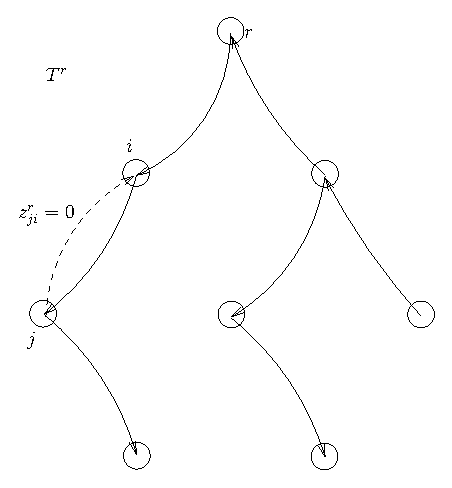
\includegraphics[scale=0.45]{figuras/variavel_u}
%%   \caption{Significado da variável $u^{r}$}
%%   \label{fig:variavel_u}
%% \end{figure}


Logo, podemos concluir que
para $j \in V$, o valor de $u^r_j$ corresponde exatamente à distância entre
$r$ e $j$ em $T^{r}$.

A validade de (\ref{res_lab:dist_bound}) pode ser vista das seguintes implicações:

\begin{itemize}
\item $z^r_{ij} = 1, z^r_{ji} = 0 \Rightarrow u^r_i + w_{ij} \le u^r_j$;
\item $z^r_{ij} = 0, z^r_{ji} = 1 \Rightarrow u^r_i \le u^r_j + w_{ij}$;
\item $z^r_{ij} = 0, z^r_{ji} = 0 \Rightarrow u^r_i - u^r_j \le M^{r}_{ij}$. 
\end{itemize}

A validade de (\ref{res_lab:dist_bound2}) segue das seguintes implicações:

\begin{itemize}
\item $z^r_{ij} = 1 \Rightarrow u^r_i \le w_{ij}$;
\item $z^r_{ij} = 0 \Rightarrow u^r_i \le M^{r}_{ir}$.
  \end{itemize}

Juntando todas as restrições mencionadas, obtemos a seguinte formulação,
denominada \emph{com rótulos} (CR), para o MWTSP:

\pagebreak

  \begin{lpformulation} %[{\rm (2)}]
    \lpobj*{min}{\sum_{e\in E} w_ex_e}
    \lpeq[]{\sum_{e \in E}x_e = |V| - 1}{}
    \lpeq[]{\sum_{i \in \delta^{-}(j)}z^{r}_{ij} = 1}{r \in V,\,\forall j \in V \setminus \{r\}}
    \lpeq[]{\sum_{i \in \delta^{-}(r)}z^{r}_{ir} = 0}{r \in V}
    \lpeq[]{x_e = z^{r}_{ij} + z^{r}_{ji}}{r \in V,\, \forall e = \{i,j\} \in E}
    \lpeq[]{u^{r}_{i} - u^{r}_{j} + (M^{r}_{ij} + w_{ij}) z^{r}_{ij} + (M^{r}_{ij} - w_{ij})z^{r}_{ji} \le M^{r}_{ij}}{r \in V, \forall ij \in A, j \ne r}
    \lpeq[]{u^{r}_{i} + (M^{r}_{ir} - w_{ir}))z^r_{ri} \le M^{r}_{ir}}{r \in V, \forall ri \in A}
    \lpeq[]{u^{r}_{r} = 0}{r \in V}
    \lpeq[res_lab:spanner]{u^{j}_{i} = u^{i}_{j} \le t \cdot w_{ij}}{ij \in E}
    \lpeq[]{x \in \espacoXBinary, z^{r} \in \espacoYBinary, u^{r} \in \espacoUuni}{r \in V}
\end{lpformulation}
  Na restrição (\ref{res_lab:spanner}), para $ij \in E$, como sabemos que
  $E(\widetilde{T}^{i}) = E(\widetilde{T}^{j})$ pelo
  Fato~\ref{afirm:arv_geradora}, podemos impor a igualdade
  $u^{j}_{i} = u^{i}_{j}$;  a restrição de desigualdade é óbvia. 

%% Ressaltamos o fato de que não encontramos na literatura formulações
%% lineares para o problema MWTSP. Assim, consideramos que a formulação
%% que apresentamos é de interesse na literatura. Realizamos alguns
%% testes computacionais, mas ainda pretendemos investir mais nisso. 

\subsection{Inequações válidas}
Quando as arestas têm peso unitário, a seguinte inequação é válida: 

\begin{align}
  \label{ineq:aresta-cam_longo}
  u^{r}_{v} + z^{r}_{rv} \ge 2, \: \forall r \in V, \forall v \in V \setminus \{r\}. 
\end{align}
A inequação~(\ref{ineq:aresta-cam_longo}) diz que para um par de vértices $r,v$ que 
define uma aresta, ou a aresta $uv$ pertencerá à solução ou o caminho entre $r$ e $v$ 
na solução será maior ou igual a dois.


%\section{Publicações}
% \label{sec:publicacoes}

\bigskip
\medskip


Finalizamos este capítulo mencionando que as duas formulações lineares
inteiras para o MWSTP, acima apresentadas, constam do
trabalho~\cite{Braga2017}, que apresentamos  no \emph{II Encontro de Teoria
  da Computação (ETC 2017)}.
         %     Nós também tivemos um resumo aceito na \emph{Euro 2018 (29th
        %       European Conference On Operational Research}), entitulado
        %     ''LP formulations and computational experiments on spanner
        %     problems''. Apesar de aceito, nós optamos por não ir apresentar o
        %     trabalho nesta conferência.          
        % }

